\documentclass[tikz,border=10pt]{standalone}
\usepackage{tikz}
\usepackage{xcolor}

\begin{document}

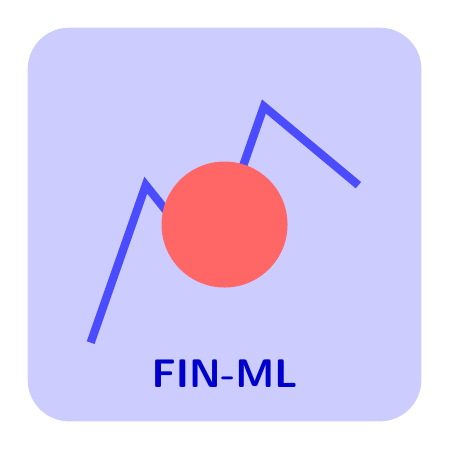
\begin{tikzpicture}

% Fond du logo
\fill[rounded corners=15pt, fill=blue!20] (0,0) rectangle (5,5);

% Graphique financier stylisé
\draw[line width=3pt, blue!70] (0.8,1) -- (1.5,3) -- (2.3,2) -- (3,4) -- (4.2,3);

% Cercle pour la barre transversale
\fill[red!60] (2.5,2.5) circle (0.8);

% Texte
\node[text=blue!80!black, font=\sffamily\bfseries\Large] at (2.5,0.6) {FIN-ML};

\end{tikzpicture}

\end{document}
